%
% Chapter 3
%

\chapter{LHC and the CMS detector}
\label{experiment}

\section{Introduction}

The prime goals of the LHC and the CMS~\cite{Chatrchyan:2008aa} experiment are exploring the physics at the~\TeV scale and studying the mechanism of electroweak symmetry breaking, including studying the SM Higgs boson's properties along with searches for new particles predicted by beyond the SM theories. The physics program's other main interests include studying the SM top quark properties, electroweak physics, and physics of hadrons containing a charm or bottom quark. Heavy-ion collisions address the physics of strongly interacting matter and the quark-gluon plasma. Hadrons consist of quarks and gluons; therefore, two colliding partons' initial energy is not known. In contrast, the collision energy is known at lepton colliders, where each particle has the same energy. Thus, hadron colliders can explore a wide range of collision energies, while lepton colliders are well suited for precision measurements.

\section{The Large Hadron Collider}
\label{sec:LHC}

The LHC is a hadron accelerator located at CERN. The design was intended to collide proton beams with a beam energy of 7~\TeV leading to a center-of-mass energy $\sqs = 14 \TeV$ and reach a luminosity of $10^{34}~\lumi$. Lead ions can be accelerated up to an energy of 2.8~\TeV per nucleon and reach a luminosity of $10^{27}~\lumi$. The LHC is the most powerful tool for particle physics research that is currently available. The 26.7 km tunnel constructed between 1984 and 1989 for the Large Electron-Positron collider~\cite{Electron-Positron:1997351} was reused to install the LHC. There are eight arcs and eight straight sections lying 45-170~\m below the surface. Unlike particle-antiparticle colliders that can use a single ring for both beams, the LHC uses two rings with counter-rotating beams. There is less synchrotron radiation owing to the heavier particles being collided at the LHC.

The accelerator complex acts as an injector of the protons and heavy ions. Protons are obtained from hydrogen gas after the electrons are stripped off, and they enter the Linear accelerator 2~\cite{accelerator:1997427}, where they are accelerated to 50~\MeV. They are further accelerated in the Proton Synchrotron Booster~\cite{Synchrotron:1997372} to 1.4~\GeV. They are then injected in the Proton Synchrotron~\cite{Synchrotron:1997189}, where they are accelerated to 25~\GeV. A bunch train is produced within the Proton Synchrotron before extraction. The protons are then accelerated in the Super Proton Synchrotron~\cite{Synchrotron:1997188} to 450~\GeV before injecting in the LHC.

The four interaction points are equipped with particle detectors: the CMS experiment, the ``A Toroidal LHC ApparatuS'' ATLAS experiment~\cite{Aad:2008zzm}, the ``A Large Ion Collider Experiment'' ALICE experiment~\cite{Aamodt:2008zz}, and the ``LHC beauty'' LHCb experiment~\cite{Alves:2008zz}. Two further smaller experiments, the ``Total Cross Section, Elastic Scattering and Diffraction Dissociation'' TOTEM~\cite{Anelli:2008zza} and the ``LHC forward'' LHCf~\cite{Adriani:2008zz} experiments, are located near the CMS and the ATLAS interaction points, respectively.

The ATLAS and CMS experiments have both multi-purpose detectors installed. The detectors were built to detect particles from \pp or heavy-ion collisions. One of the main tasks currently is to study the production and decay of the discovered Higgs boson~\cite{Chatrchyan:2013lba}, disentangle its properties, and check if it is the SM Higgs boson or a Higgs boson of an extension of the SM. The other tasks involve high precision tests of QCD, electroweak interactions, and heavy flavor physics. Precision measurements of production, the couplings, and the spin of the top quark are also pursued. Several searches for supersymmetric particles and dark matter are also ongoing.

During the LHC Run 2 data-taking, a bunch spacing of 25~\ns was used, and \pp collision data were collected at $\sqs = 13 \TeV$ in 2016, 2017, and 2018. The integrated luminosity delivered to CMS as a function of time is shown in Figure~\ref{fig:lumi} for each \pp collision data-taking period. CMS does not record the whole delivered data, and only part of the recorded data that is considered good is used for physics analysis.

\begin{table}[!hbpt]
  \centering
  \caption{Integrated luminosity considered for physics analysis at the CMS experiment during Run 2}
  \begin{tabular}{|c|c|}
    \hline Year & Integrated luminosity \\
    \hline 2016 & 35.9~\fb \\
    \hline 2017 & 41.5~\fb \\
    \hline 2018 & 59.3~\fb \\
    \hline
  \end{tabular}
  \label{tab:luminosity}
\end{table}

\begin{figure}[htbp]
  \centering
  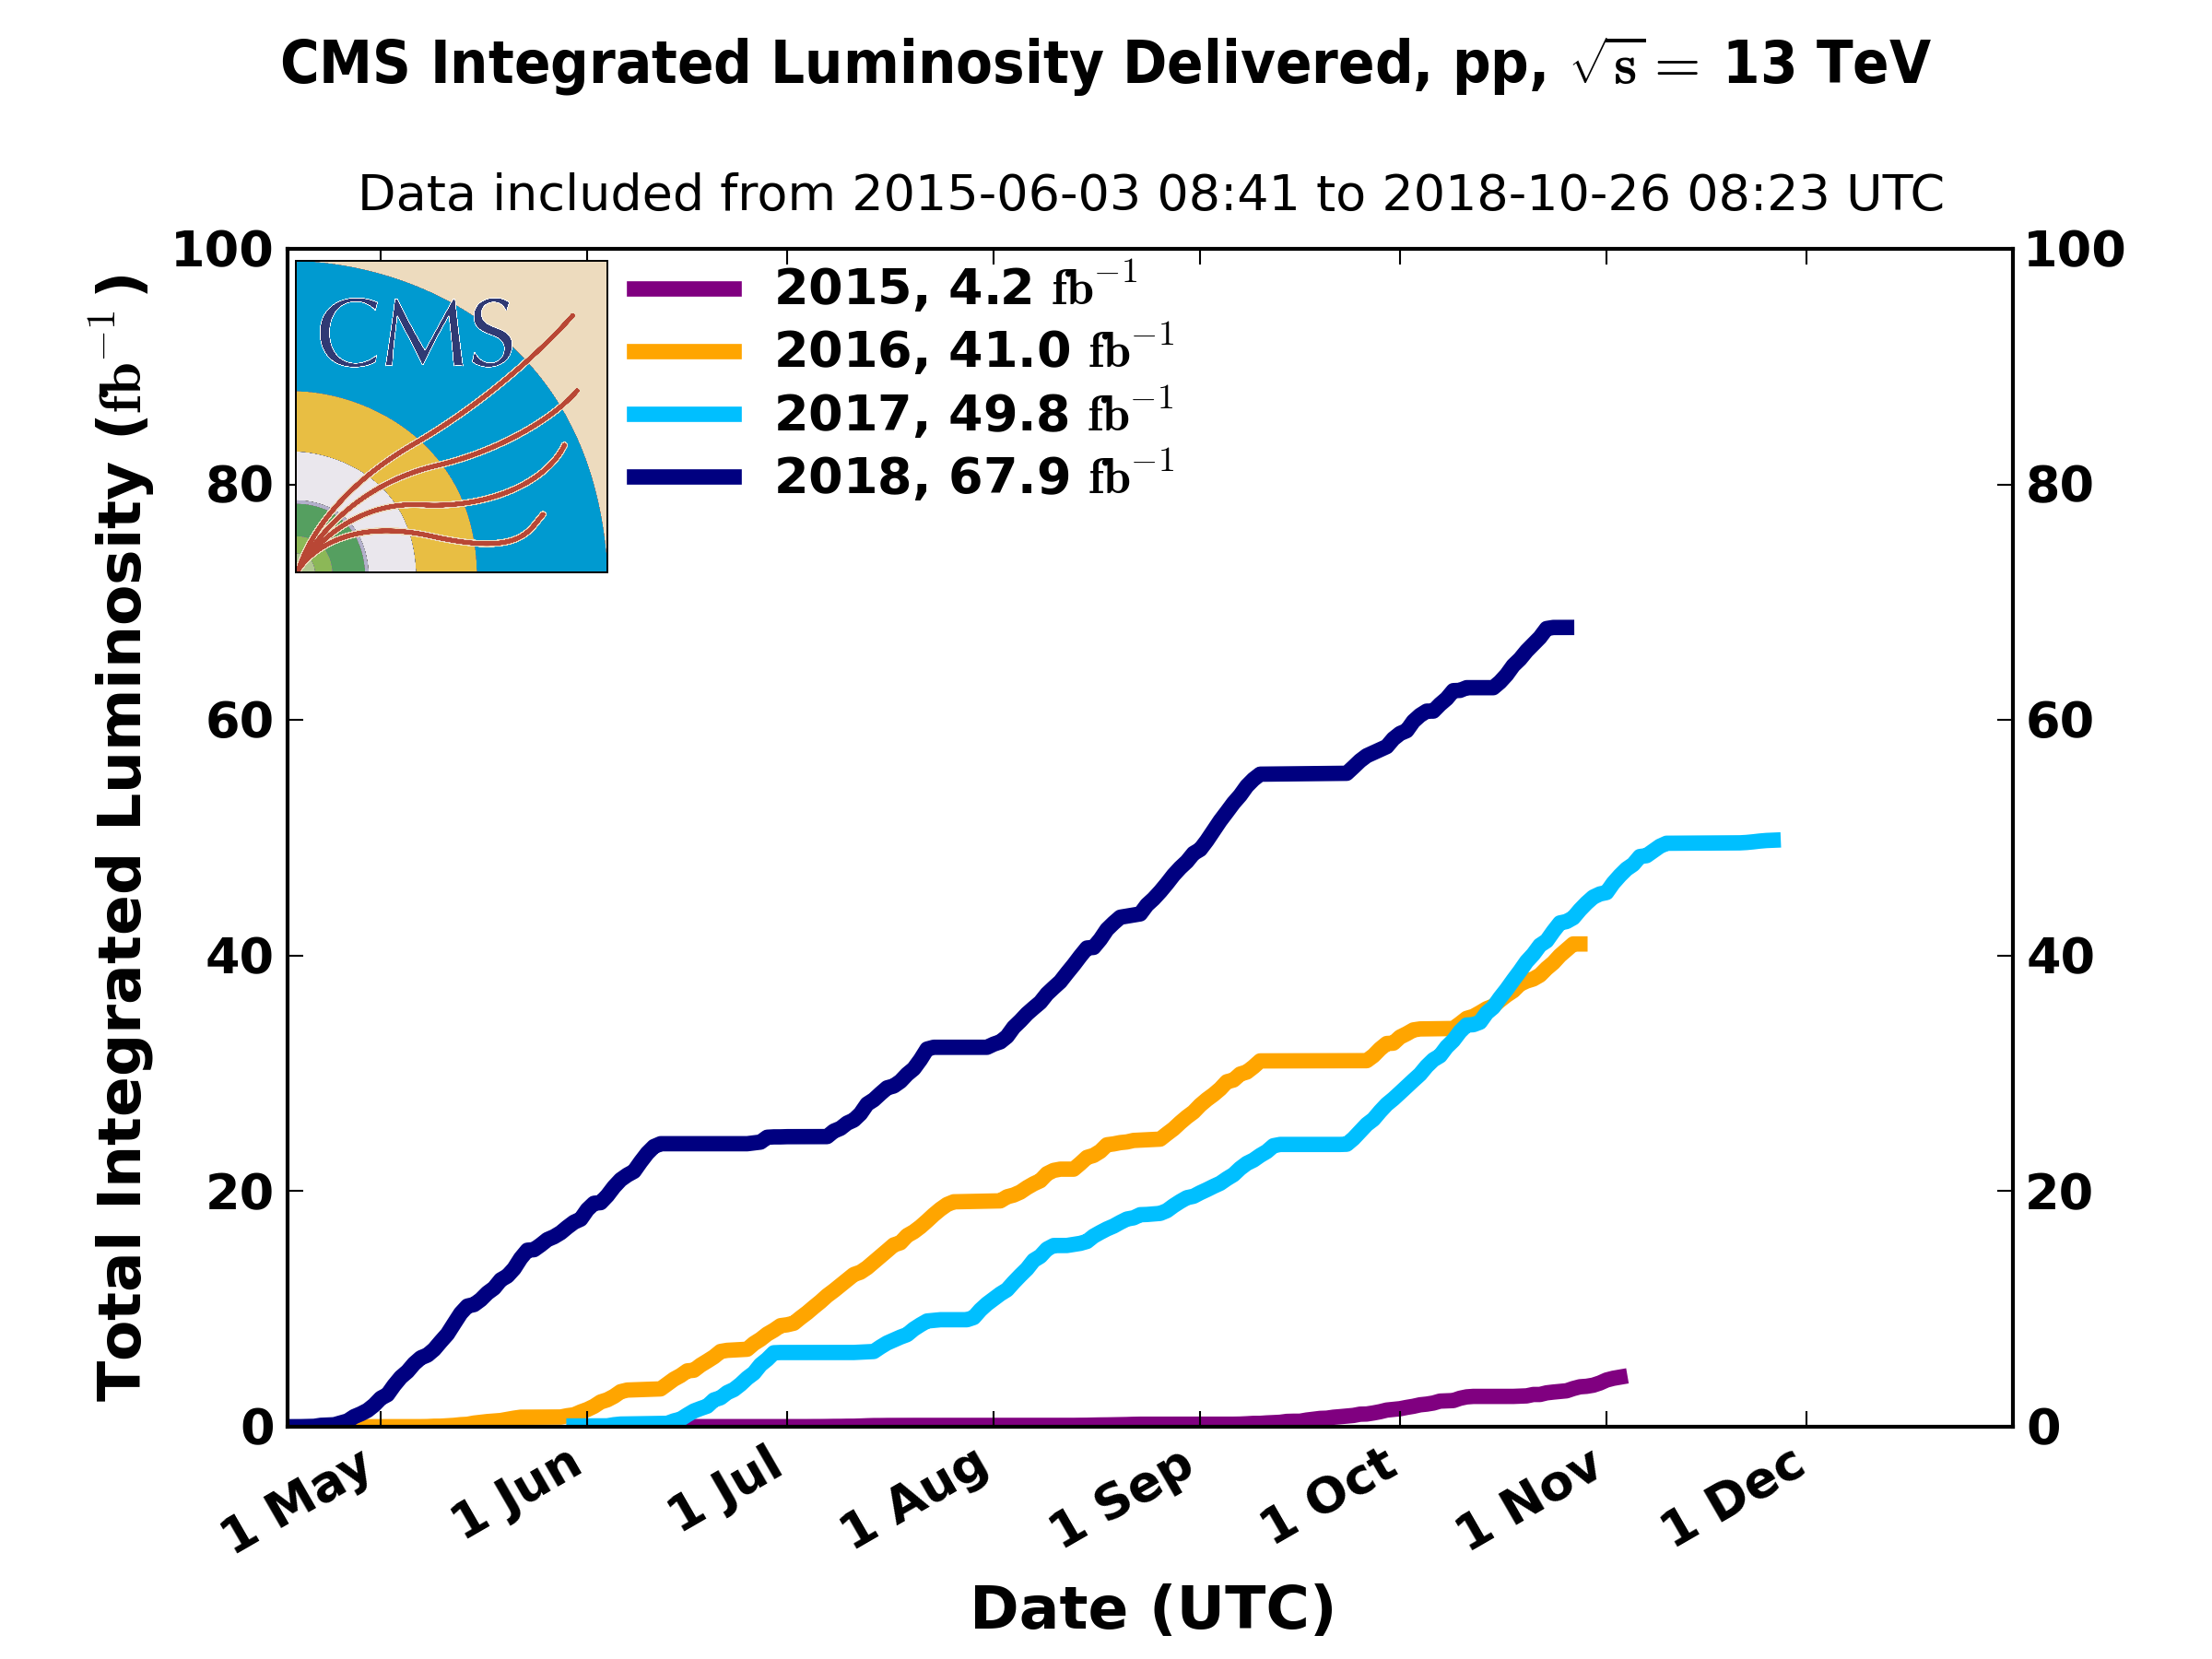
\includegraphics[width=0.8\textwidth]{plots/chapter3/int_lumi.png}
  \caption{Cumulative luminosity as a function of time delivered to CMS during stable beams for \pp collisions. The luminosity is shown for 2015 (purple), 2016 (orange), 2017 (light blue), and 2018 (dark blue)~\cite{lumi}.}
  \label{fig:lumi}
\end{figure}

\section{The Compact Muon Solenoid experiment}
The layout of the CMS detector is shown in Figure~\ref{fig:cms}. As the name ``Compact Muon Solenoid'' indicates, a superconducting solenoid is at the heart of CMS. A considerable bending power for the momentum measurement of charged particles within a compact design is achieved using a high magnetic field of 3.8 T. The internal part of the solenoid is large enough to accommodate the inner tracking system and the calorimetry. The inner tracking system is composed of a pixel detector close to the interaction region and a silicon strip tracker. The pixel detector can resolve individual vertices and distinguish between vertices from the primary interaction and secondary vertices from the decay of the primary interaction particles. The trajectories are precisely measured with the high granular silicon strip tracker, which can deal with high charged particle multiplicities.

\begin{figure}[htbp]
  \centering
  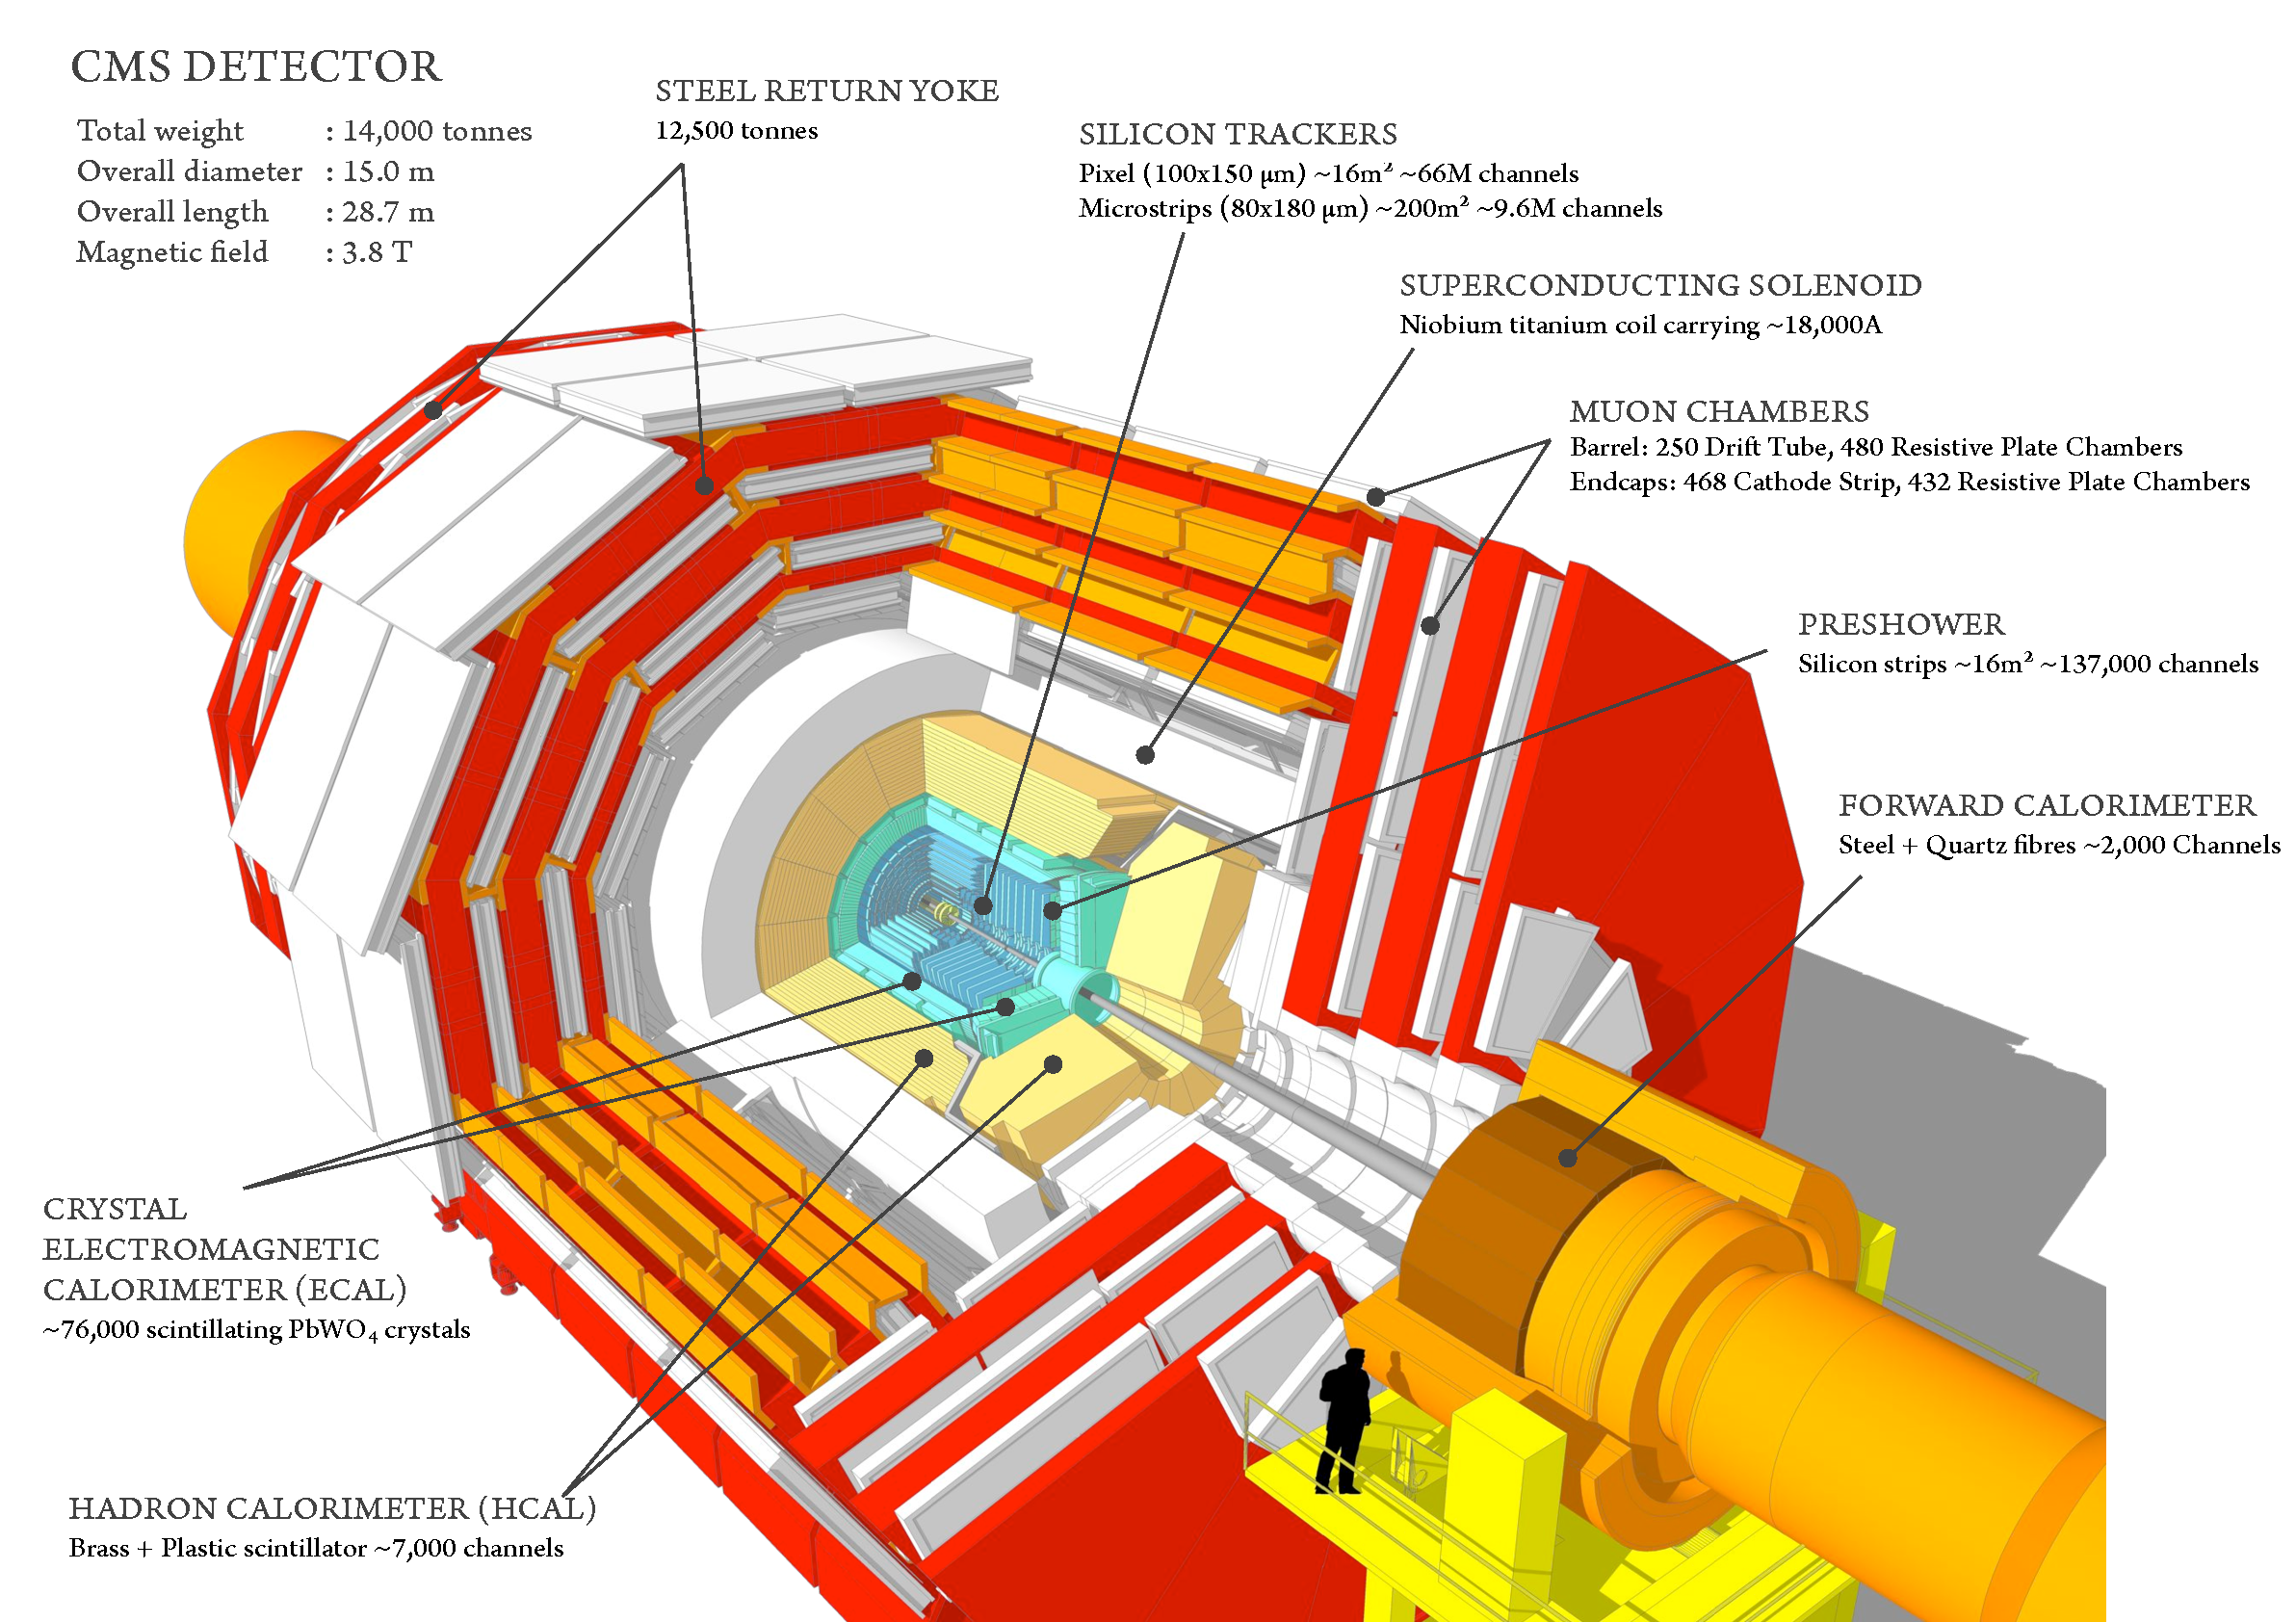
\includegraphics[width=0.9\textwidth]{plots/chapter3/cms_layered.png}
  \caption{Schematic view of the CMS detector.}
  \label{fig:cms}
\end{figure}

The energy of the particles is measured in calorimeters. The calorimeter material initiates electromagnetic or hadronic showers. For electromagnetic interactions, the characteristic interaction length is the radiation length $X_0$, while the characteristic interaction length for hadronic showers is the nuclear interaction length $\lambda_I$. The entire volume is sensitive in homogeneous calorimeters, while sampling calorimeters consist of metallic absorber sandwiched or threaded with an active material that generates the signal. CMS has an electromagnetic calorimeter (ECAL) made of lead tungstate ($\text{PbWO}_{4}$) crystals in front of a brass/scintillator sampling hadron calorimeter (HCAL). An additional layer of scintillators is outside the coil. The magnet is used as an absorber material. This iron/quartz-fiber calorimeter is referred to as the hadron outer detector. The muon detectors are sandwiched between the layers of the steel return yoke. Their main task is to trigger on muons and to identify the muons with good momentum resolution.

\subsection{The coordinate system of CMS}
The CMS experiment uses a right-handed coordinate system, with the origin at the nominal collision point. The x-axis points towards the LHC center, while the y-axis points upward towards the surface (perpendicular to the LHC plane), and the z-axis points along the anti-clockwise beam direction. Two angles are defined, where the azimuthal angle $\phi$ is measured from the x-axis in the x-y plane, and the polar angle $\theta$ is measured from the z-axis. Pseudorapidity is defined as

\begin{equation}
  \eta=-\ln \left[\tan \left(\frac{\theta}{2}\right)\right]
\end{equation}

and describes the angle of a particle relative to the beam axis, illustrated in Figure~\ref{fig:coordinate}. Distances in $\phi$ and $\eta$ are denoted $\Delta\phi$ and $\Delta\eta$. These distance measures are used to define the spatial separation between physics objects by \dr with

\begin{equation}
  \dr=\sqrt{(\Delta \phi)^{2}+(\Delta \eta)^{2}}
\end{equation}

\begin{figure}[htbp]
  \centering
  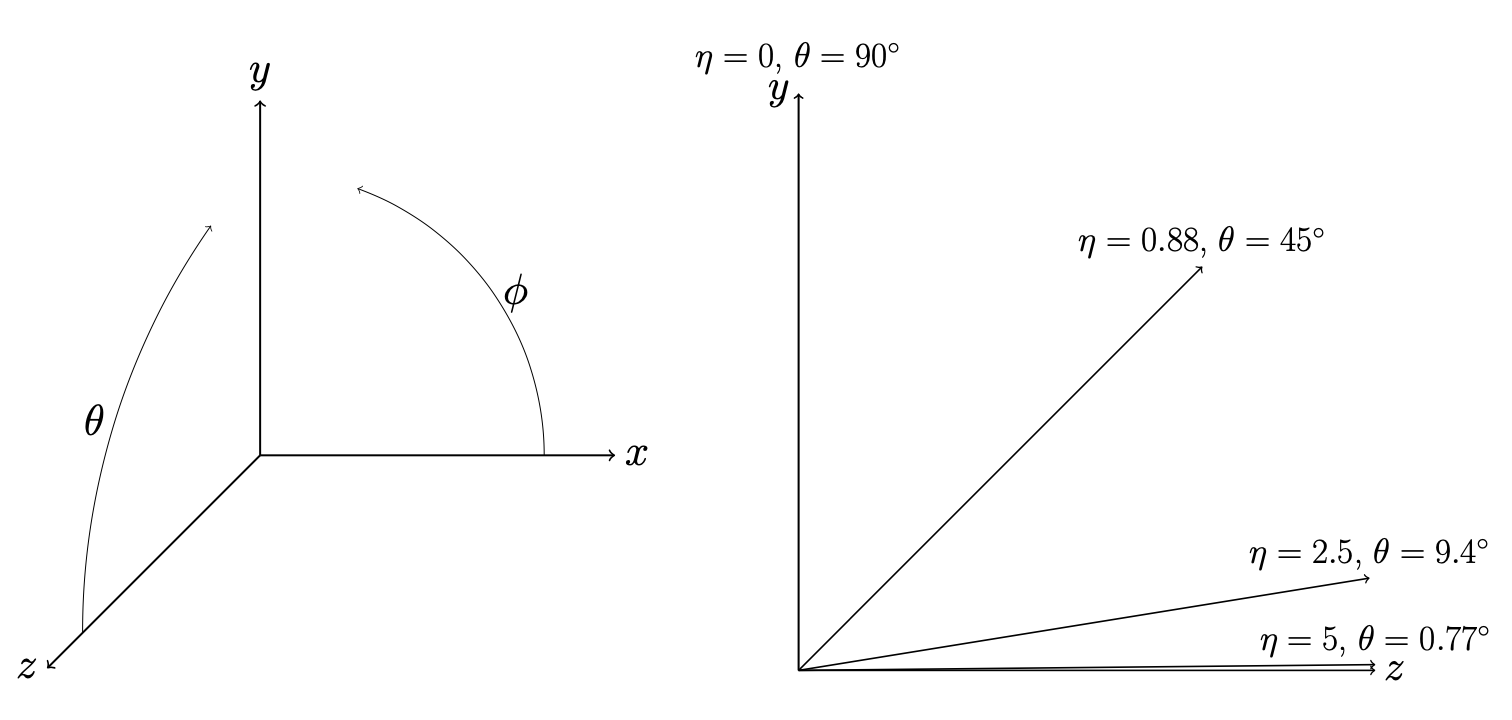
\includegraphics[width=0.9\textwidth]{plots/chapter3/coordinate.png}
  \caption{Coordinate system convention of CMS (left) and the relation between pseudorapidity $\eta$ and polar angle $\theta$ (right)}
  \label{fig:coordinate}
\end{figure}

\subsection{Kinematic quantities}
At LHC, the protons carry half of the collision energy. The hard interactions occur between the colliding protons' partons, and each parton carries a fraction $x_i$ of the proton momentum. As the parton mass can be neglected with respect to the momentum $\vec{p}$, the parton energy is given by its momentum. In the laboratory frame, the four-momenta of the partons are

\begin{equation}
  \begin{aligned}
    \text{p}_{1}&=x_{1} \cdot \frac{\sqs}{2}(1,0,0,1) \\
    \text{p}_{2}&=x_{2} \cdot \frac{\sqs}{2}(1,0,0,-1)
  \end{aligned}
\end{equation}

Then, the invariant mass of the hard collision is given by

\begin{equation}
  \hat{s} \equiv \text{M}^{2}=\left(\text{p}_{1}+\text{p}_{2}\right)^{2}=\frac{s}{4} \cdot\left[\left(x_{1}+x_{2}\right)^{2}-\left(x_{1}-x_{2}\right)^{2}\right]=x_{1} x_{2} s
\end{equation}

where $\sqrt{\hat{s}}$ denotes the center-of-mass energy of the parton-parton collision. The hard collision products have a zero total momentum for the x- and y-components but in general non-zero for the z-component. Thus, the hard-collision products' momentum and energy are measured transverse to the beam direction in the x-y plane. The transverse momentum is denoted by \pt and the transverse energy is denoted by \ET with $\ET = \text{E} \cdot \text{sin} \theta$. The weakly interacting particles, like neutrinos, do not produce a signal in the CMS detector and lead to an imbalance in the observed total transverse momentum in the event, missing transverse energy, denoted as \met.

\subsection{Detector requirements}
Isolated leptons in the final states leave clean signatures in the CMS detector. The muon has to be well-identified, and its momentum resolution needs to good over a wide range of momenta. The charge of the muon has to be determined unambiguously. In addition, electrons and charged hadrons need to be reconstructed and identified with good efficiency and momentum resolution. The momenta of charged particles are measured using the curvature of their trajectory. Hence, considerable bending power is needed to measure precisely the charge of particles with large momentum. Furthermore, a good electromagnetic energy resolution is needed over a wide geometrical coverage and correct localization of the primary interaction.

The CMS detector can detect the hadrons produced from the hadronization of the quarks. Tau leptons that decay hadronically need to be identified with good efficiency for the Higgs boson physics. A good measurement of the impact parameter of charged particle tracks and good position measurement of the secondary vertices can improve the triggering and identification efficiency of hadronically decaying taus. This requires having the pixel detector close to the interaction region. Hadronic calorimeters with a large hermetic coverage ($\aeta < 5$) and with a fine lateral segmentation $(\Delta \eta \times \Delta \phi < 0.1 \times 0.1)$ are required for measuring the hadrons energy with good resolution and for the estimation of \met.

The collisions are happening at a rate of 40~\mhz and not all of these events can be stored; therefore, only interesting events have to be selected. The online event selection process, trigger, must reduce the rate to $\sim 1~\khz$. The short time between two bunch crossings, 25~\ns, has a major implication on the read-out and trigger system design. Multiple \pp interactions (pileup) happen in one bunch crossing. The interactions' products overlap and can be wrongly linked, and long response times of detector elements and their electronic signal longer than 25~\ns increase this effect. High granularity detectors with good time resolution result in a low occupancy. This requires many detector channels and, therefore, a good synchronization of the electronic detector channels. The large flux of the particles and resulting high radiation levels require radiation-hard detectors and front-end electronics.

\subsection{Magnet}

The curvature of the particle trajectory in a magnetic field determines the momenta and sign of charged particles. The most important aspect of muon measurement is the choice of magnetic field configuration. A good momentum resolution of $\Delta \text{p} / \text{p} \approx 10 \%$ is required for muons with a momentum of 1~\TeV. CMS uses a large superconducting solenoid with a magnetic field of 3.8 T. The solenoid is 13 m long and has an inner diameter of 5.9 m. The superconductor material is Niobium-titanium~\cite{BUL-NA-2003-150}. The conductor is made of high purity and is aluminum stabilized with a four-layer winding and is composed of five coils and has to withstand outward pressure. The superconducting wire is cooled using an indirect cooling by thermosyphon.

\subsection{Inner tracking system}

The inner tracking system~\cite{Khachatryan:2010pw} measures the trajectories of particles up to $\aeta < 2.5$. The particle flux is the highest close to the interaction region. The silicon pixel detector is placed close to the interaction region. This allows for the reconstruction of vertices from heavy flavor hadrons with a b or c quark. Each pixel has a size of $\approx 100 \times 150 \mum^{2}$. The spatial resolution of the radius and azimuthal angle $r$--$\phi$ measurement is about 10~\mum and 20~\mum for the $z$-coordinate measurement. In the intermediate region ($20 < r < 55 \cm$) and outermost region ($r > 55 \cm$) silicon microstrips are used with a size of $10 \cm \times 80 \mum$ (minimum cell size) and a size of $25 \cm \times 180 \mum$ (maximum cell size), which provide the required granularity. The barrel's tracking volume has a cylindrical shape with a length of 5.8~\m and a diameter of 2.6~\m. The pixel detector consists of three layers at radii of 4, 7, and 11~\cm in the barrel.

Additionally, there are ten layers of silicon microstrip detectors. The strip tracker is divided into a tracker inner barrel (TIB) made out of four layers and a tracker outer barrel (TOB) made out of six layers. Each part has two layers which provide a single-point measurement in the $r$--$\phi$ and $r$--$z$ coordinates. In the TIB, the single-point resolution is 23--34~\mum in the $r$-direction and 23~\mum in $z$, while it is 35--52~\mum in the $r$--$\phi$ direction and 52~\mum in $z$ for the TOB. In the two end caps, there are just two-pixel layers and nine microstrip layers. The strip tracker's endcaps are divided into the tracker endcap made of 9 disks and the tracker inner disks made of three small disks, which fill the gap between the TIB and the tracker endcap.

\subsection{Electromagnetic calorimeter}

The ECAL is a hermetic, homogeneous calorimeter with a coverage of $\aeta < 3$, and it measures the energy of electrons and photons. It has an excellent energy resolution and high granularity and can separate close clusters very well~\cite{CMS:2010bta, Khachatryan:2015hwa}. ECAL uses $\text{PbWO}_4$ crystals, which have a short radiation length of $X_0 = 0.89 \cm$. These crystals are radiation hard and emit blue-green scintillation light with a maximum at 420 nm. The crystals allow a compact calorimeter inside the solenoid that is fast, has a fine granularity and is radiation-resistant. The decay time for the scintillation is short and in the same order as the LHC bunch crossing time, and about 80\% of the light is emitted within 25~\ns. However, the light output depends on the temperature. Therefore, to preserve energy resolution, a cooling system is needed. Besides, as the light yield is low, this requires photodetectors with intrinsic gain that can also operate in a high magnetic field. Figure~\ref{fig:ecal} illustrates the layout of the ECAL.

\begin{figure}[htbp]
  \centering
  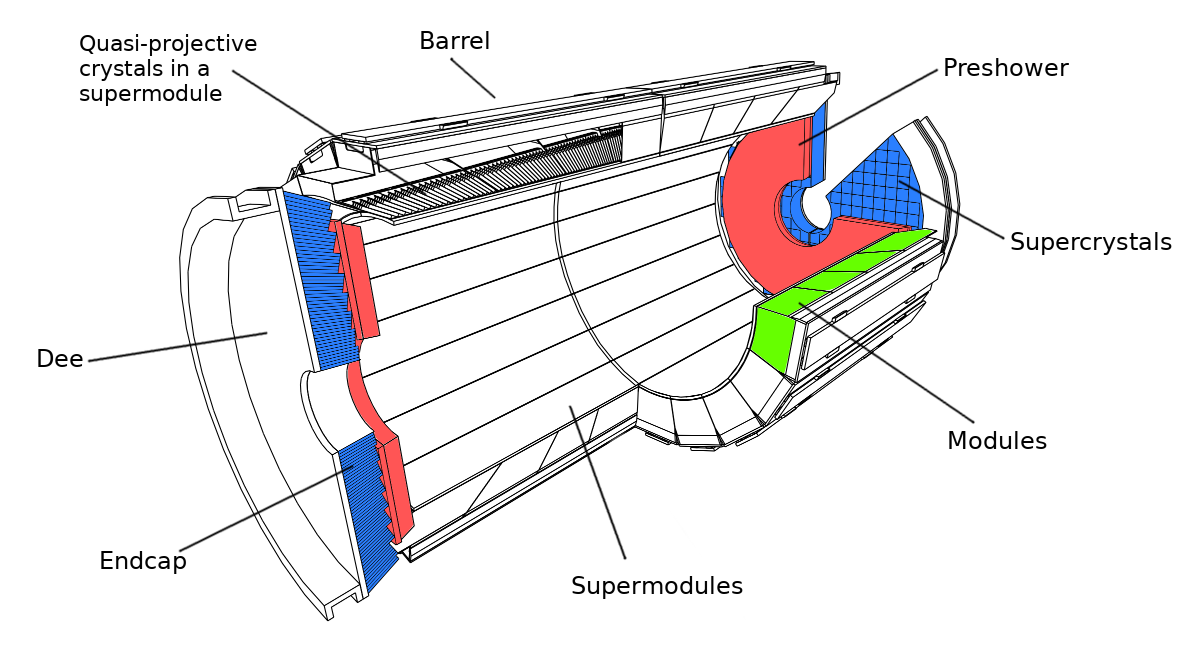
\includegraphics[width=0.9\textwidth]{plots/chapter3/ecal.png}
  \caption{Schematic view of the ECAL.}
  \label{fig:ecal}
\end{figure}

The calorimeter is divided into a ECAL barrel (EB) which covers the region $0 < \aeta < 1.479$ and two ECAL endcaps (EE) which cover the region $1.479 < \aeta < 3.0$. Preshower detectors are installed in front of each endcap and cover the region $1.653 < \aeta < 2.6$. In the EB, the scintillation light is detected with silicon avalanche photodiodes (APD). These photodiodes respond to temperature changes and require a stable temperature. The barrel section is structured in 36 identical supermodules, 18 in each half barrel, with the crystals being arranged in a grid and covering $\Delta \eta \times \Delta \phi = 0.0174 \times 0.0174$. In the EE, the scintillation light is detected with vacuum phototriodes. A $5 \times 5$ array of crystals is termed supercrystals. The crystals and the supercrystals are arranged in a rectangular x-y grid. The preshower system is installed in front of EE to identify and reject $\pi^0$ mesons, which dominantly decay into two photons. It has a higher granularity than the EE and improves the position determination of electrons and photons. It is a sampling calorimeter consisting of two layers of a lead absorber, which initiate the electromagnetic showers from incoming electrons or photons. The lead radiators are followed by silicon strip sensors measuring the energy deposits and the transverse shower profiles. The silicon strip sensors are oriented orthogonally and are placed after a radiation length of 1 $X_0$ and 2 $X_0$ of the lead absorber.

The ECAL calibration and performance is estimated from the supercluster energy deposited by the electrons and photons. The calibration is performed, which corrects the detector's response to the energy deposited to match expectations. The calibration is applied to the superclusters to take into account the $\eta$ and $\phi$-dependent geometry and material effects, as well as the fact that electrons and photons shower slightly differently. The calibrations were tuned and validated using electrons' energy from \PW boson decays, the reconstructed mass from $\eta$ decays to two photons, and the energy resolution measured with \Zee events. I implemented an event skimmer using the updated electron identification and isolation selections to select events with \Zee resulting from the \pp collisions. The primary motivation for implementing the event skimmer is to obtain datasets enriched with \Zee events that can be further used for performing calibration in ECAL, and because trigger selections are not applied in the event skimmer, it can be used for trigger efficiency studies. One primary difference from the old event skimmer is using the effective area method to calculate electrons' isolation instead of the delta beta method. The description of these methods is given in section~\ref{isolation}. The event skimmer's acceptance is tested on the 2017 data, and the obtained event rate is within expectations. It is currently integrated into the CMS software framework.

\subsection{Hadron calorimeter}

The HCAL is a sampling calorimeter, and it measures the energy of hadrons. The HCAL system is located surrounding the ECAL system, and most of it is located inside the solenoid. The HCAL design has an important requirement to minimize the non-Gaussian tails in the energy resolution and to provide a good hermeticity for the determination of \met. Another design requirement is to maximize the interaction length of the material within the solenoid. This corresponds to minimizing the space allocated to the active material. It is divided into a HCAL barrel (HB) detector, covering the region $\aeta < 1.4$ and two HCAL endcap (HE) detectors, covering $1.3 < \aeta < 3.0$. The absorber material is brass. Brass is chosen because it has a relatively short interaction length, is easy to machine, and is non-magnetic. The active material is a plastic scintillator. In order to provide structural support, stainless steel is used in the innermost and outermost layers. The 3.7~\mm thick scintillator plates are sandwiched between the absorber plates. Wavelength-shifting fibers are embedded in the scintillator tiles, which channel the light to photodetectors that can operate in high axial magnetic fields called hybrid photodiodes. In the HB, the segmentation is $\Delta \eta \times \Delta \phi = 0.087 \times 0.087 \approx 5^{\circ} \times 5^{\circ}$, which is termed tower. In the HE, the $\phi$ segmentation is $5^\circ - 10^\circ$ and the $\eta$ segmentation is 0.087--0.35 depending on $\eta$.

The energy from the hadron showers that leak through the calorimeters' rear are samples with additional layers of scintillators are installed outside the coil within the return yoke using the iron as an absorber. This helps in improving the central shower containment and the \met resolution of the calorimeter. This sampling calorimeter is referred to as hadron outer detector. It is located along with the muon barrel system and closely follows its segmentation. It is divided into five sections termed rings along $\eta$. The hadron outer detector follows the HB geometry in $\eta$ and $\phi$ and covers the region $\aeta < 1.26$. Two further detectors, which cover the region $2.9 < \aeta < 5.0$, are specialized in measuring energetic forward hadronic showers and ensuring full geometric coverage for the transverse energy measurement. The HCAL forward (HF) sampling calorimeters use steel as absorber material and quartz fibers as the active material. Cherenkov light is emitted by the shower particles in the quartz fibers and is channeled to photomultipliers. The hadron showers' neutral components are preferentially sampled in the HF, leading to narrower and shorter hadronic showers, and is ideally suited for the forward region.

\subsection{Muon system}

The muon system is installed in the magnet return yokes of the CMS detector. The muon system's main task is to identify muons with good efficiency and reconstruct its momentum with good resolution and assign the correct charge even for high-\pt muons. It is also tasked with triggering events with muons. It is divided into a barrel detector covering $\aeta < 1.2$ and two endcap detectors, covering the region $0.9 < \aeta < 2.4$, defining three regions: the barrel region ($\aeta < 0.9$), the overlap region ($0.9 < \aeta < 1.2$), and the endcap region ($1.2 < \aeta < 2.4$). The muon system has three different types of gaseous detectors in different radiation environments. As the muon rate, the neutron-induced background rate, and the residual magnetic field are low in the barrel region, the drift tube (DT) chambers are used. In the two endcaps, the muon rate, the neutron-induced background, and the magnetic field are high, and hence the cathode strip chambers (CSC) are used in this region. Resistive plate chambers (RPC) are used in both subdetectors covering the region $\aeta < 1.6$. They are operated in avalanche mode to ensure good operation at high rates. The RPCs have double gaps with a width of 2 mm filled with gas. They have a fast response with a good time resolution but a coarser position resolution than the DTs and CSCs and are thus used to identify the correct bunch crossing.

Figure~\ref{fig:muon} gives an overview of the muon system's layout. The barrel is divided into four stations arranged in cylinders interleaved with the iron yoke. It is also divided into five wheels along the beam direction following the five wheels of the return yokes. There are 12 layers divided into 3 Super Layers (SL) made out of four DTs layers in each chamber. The two SL measure the $r$--$\phi$ coordinate, while a third SL sandwich between them measures the $z$ coordinate. In the last muon station, there are only two SL to measure the $r$--$\phi$ coordinate. There are one or two associated RPCs in each DT chamber. The DTs have a single point resolution of $\approx 200 \mum$. The CSCs and RPCs are arranged in four disks in each endcap. They are divided into three concentric rings in the innermost station or two concentric rings in the other stations. Up to six space coordinates $(r, \phi, z)$ are measured in each CSC, and the provided spatial resolution is $\approx 200 \mum$, except for the innermost ring in the first disk, where it is $\approx 100 \mum$. The angular resolution in $\phi$ is $\sim 10~\text{mrad}$. The DTs or CSCs and the RPCs provide two independent and complementary information sources.

\begin{figure}[htbp]
  \centering
  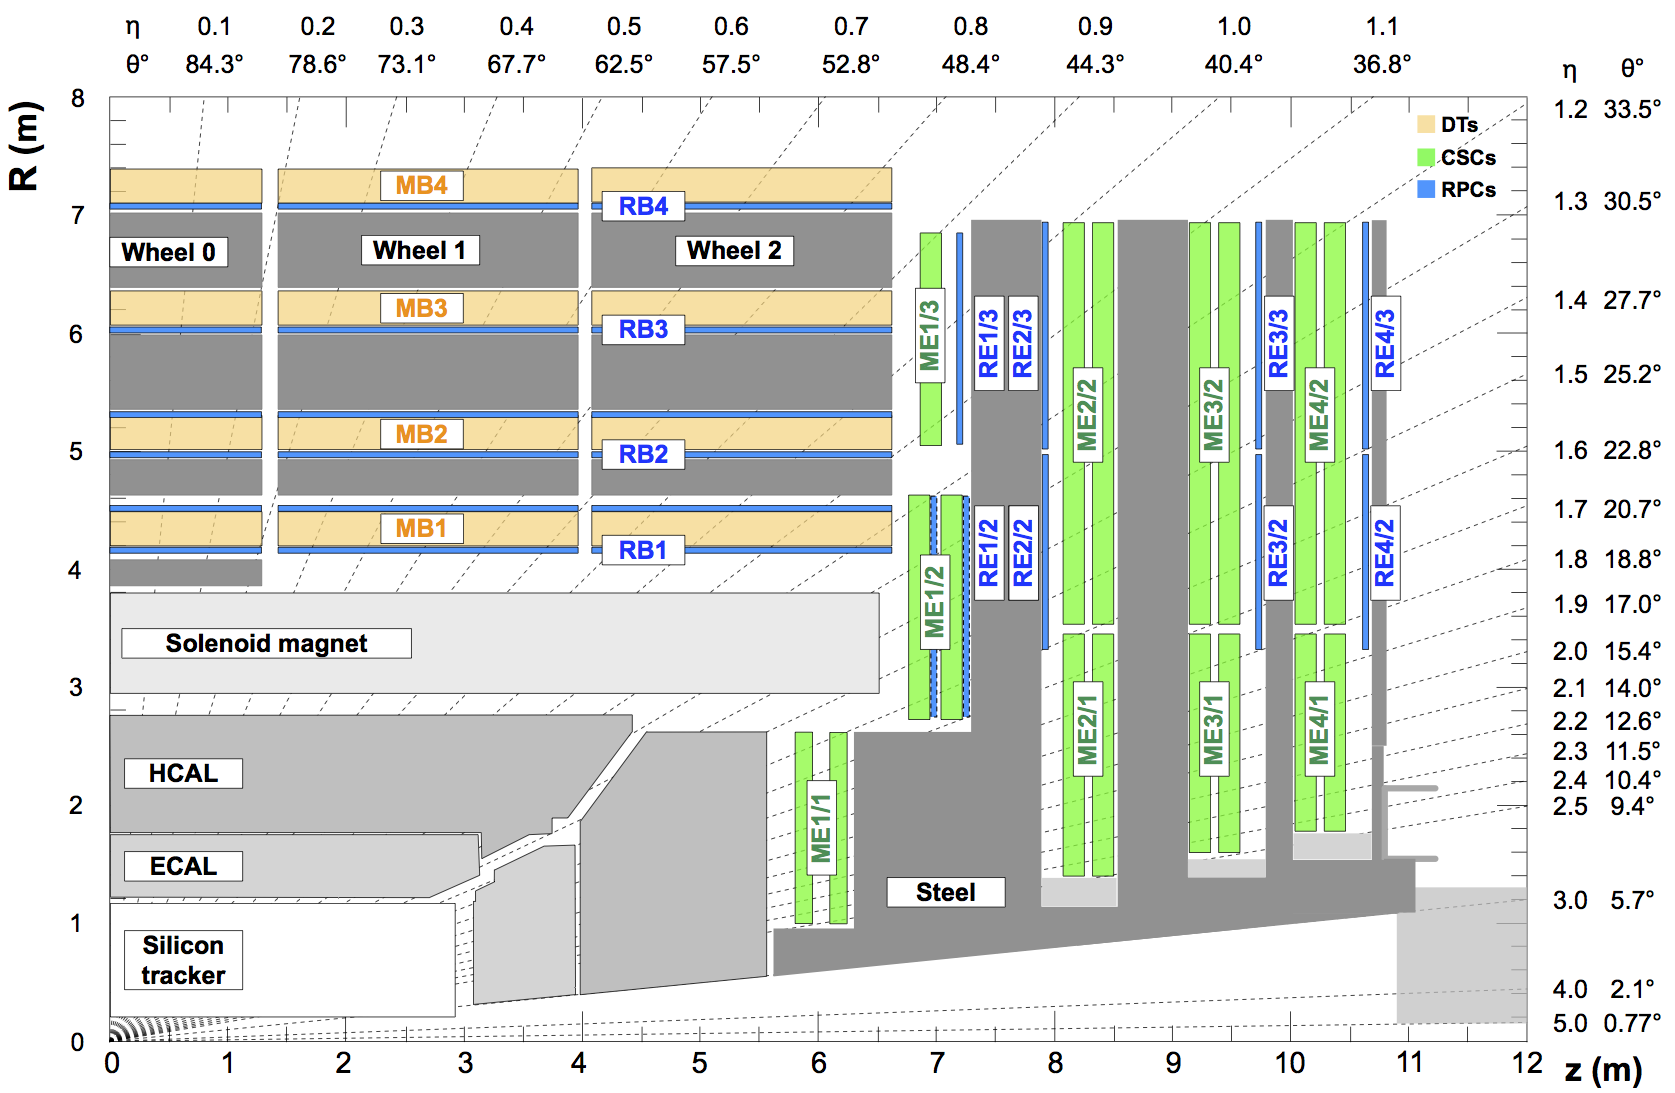
\includegraphics[width=0.9\textwidth]{plots/chapter3/muon.png}
  \caption{Schematic view of the muon detectors.}
  \label{fig:muon}
\end{figure}

\subsection{Trigger and data acquisition system}

The online event selection process, trigger, reduces the rate to about 1~\khz. First, the detector electronics detect signals and pass them to the Level-1 trigger processors. The Level-1 trigger logic is located in a service cavern and selects events of interest. Due to the size of the CMS detector and underground caverns, the transit and time needed for a decision is about 3.2~\mus, during which the data is held in pipelined memory buffers. However, the time needed for Level-1 trigger calculations is only 1~\mus. Custom hardware processors form the Level-1 decision to keep or discard data using the calorimetry, muon systems, and correlation information. Trigger primitive objects, such as electrons or muons above a set \ET or \pt thresholds are used for the decision making. Reduced granularity and resolution data are used to form the trigger objects. Sums of \ET and \met are also employed. If a decision is made to keep the event, the data is transferred to the front-end read-out buffers. The data is further processed and compressed and placed in dual-port memories.

A processor farm is responsible for filtering the events. Each processor runs the same High-Level Trigger (HLT) code, reducing the output rate from 100~\khz to 1~\khz. Using a processor farm for event filtering allows for computer technology evolution and maximizes the flexibility in selecting data and algorithms. Whenever possible, only necessary objects are reconstructed, and only needed information of some subdetectors are used. The idea of partial reconstruction and many virtual trigger levels is the basis for the HLT. First, calorimeter and muon information is used, followed by the use of pixel tracker data. Finally, the full event information is used, including full tracking. The HLT system uses identification and isolation criteria as well as minimal energy or transverse momentum thresholds.

The data acquisition path of the ECAL sub-detector will be described in the following paragraphs. The process starts when the global trigger distributes the Level-1 decision. The data concentrator card is the main ECAL read-out unit and is responsible for collecting the crystal data. It also aggregates the trigger primitive information and performs an extensive integrity check of the data received. About 100 kB per event have been allocated for ECAL data, but the full event payload, if all channels are read out, exceeds this target by a factor of nearly 20. The selective read-out processor can perform the reduction of the data volume. The suppression applied to a channel takes account of energy deposits in the vicinity to achieve the best resolution for large energy deposits~\cite{Almeida:2008zz}.

The calorimeter regions are classified into three groups by comparing the transverse energy deposited in each trigger tower with two configurable thresholds. Upon receiving the Level-1 decision, the information is transmitted to the selective read-out processor, determining the read-out mode that the data concentrator card has to apply to each trigger tower. There are two read-out modes: full read-out and zero suppression. With full read-out, the crystal time samples are saved without any suppression. With zero suppression, the signal's amplitude for each crystal is calculated by applying the finite impulse response filter over the digitalized time samples and compared with a configurable threshold: if the amplitude is above the suppression level, the crystal data is saved; otherwise, it is discarded.

I upgraded the selective read-out processor monitor from the legacy monitoring system and the error database to quickly diagnose re-appearing errors for the ECAL. The online monitoring system checks the status of various online electronic components of ECAL. The ECAL experts regularly use the new monitoring system to identify errors so that there is minimal data collection loss~\cite{Siddireddy:2018gxt}. Figure~\ref{fig:SRP} shows the online monitoring system in operation during data-taking.

\begin{figure}[htbp]
  \centering
  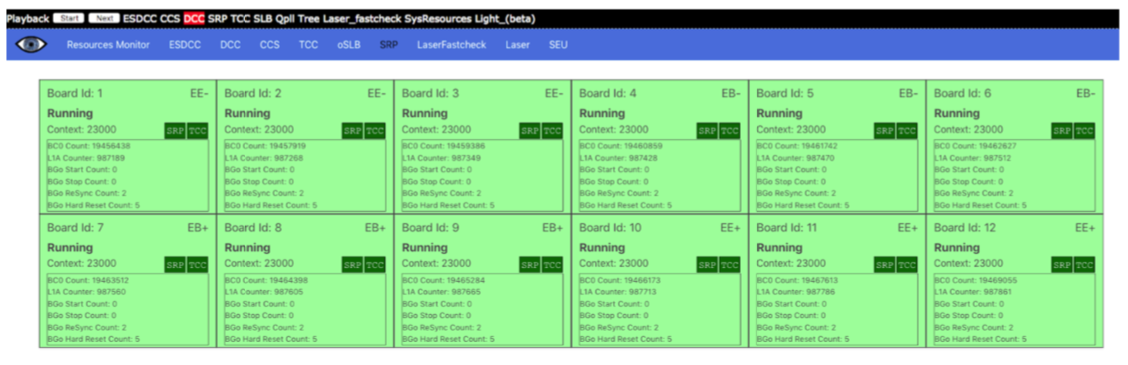
\includegraphics[width=0.9\textwidth]{plots/chapter3/SRP.png}
  \caption{The ECAL electronics online monitoring system in operation.}
  \label{fig:SRP}
\end{figure}

\subsection{Luminosity measurement}

Luminosity is defined as the ratio of the event rate to the cross-section of a given process. It is the effective area quantifying the likelihood of a scattering event. The cross-section is measured in units of area, thus the luminosity is given in units of events per time per area, $(b.s)^{-1} = 10^{24}~\lumi$. The integrated luminosity is the integral over the instantaneous luminosity $\text{L}=\int \mathcal{L}(t) dt$. The number of expected events for a given process is given by the product of the integrated luminosity and the production cross-section, $\mathrm{N_{exp}}=\text{L} \cdot \sigma_{exp}$.

The performance of LHC is monitored in real-time using luminosity measurements and they provide an overall normalization for physics analyses~\cite{Bayatian:2006nff}. The cross-section of a given process can be estimated using a reference process, $\sigma_{\exp} = \frac{N_{\exp}}{N_{\text{ref}}} \cdot \sigma_{\text{ref}}$, where $N_{\text{ref}}$ and $\sigma_{\text{ref}}$ are the number of reference events and the reference process's cross-section. The above equation assumes that the same integrated luminosity has been used for both processes. The modern colliders use bunched beams~\cite{Tanabashi:2018oca}. If two bunches with $n_1$ and $n_2$ particles collide head-on with frequency $f$, then the instantaneous luminosity is given by:

\begin{equation}
  \mathcal{L}=f \cdot \frac{n_{1} n_{2}}{\sqrt{\epsilon_{x} \beta_{x}^{*} \epsilon_{y} \beta_{y}^{*}}}
\end{equation}

where ${x,y}$ are the beams transverse coordinates, $\beta^*_{x,y}$ are the interaction points amplitude functions, where the beam optics produce a narrow focus. Emittance is a measure of the beam width defined as $\epsilon_{x} \equiv \frac{\sigma_{x}^{2}}{\beta_{x}}$, with the root mean square of the transverse beam sizes in the horizontal or vertical direction being $\sigma_{x}$ and $\sigma_{y}$, respectively. The instantaneous luminosity can be increased by colliding bunches with a high population of low emittance at high frequency at locations where the beam optics provide low values of the amplitude functions. As the beam parameters change, the instantaneous luminosity has to be measured correspondingly.

The event rate of a reference process can estimate the instantaneous luminosity if the cross-section is known. The visible cross-section is given by: $\sigma_{\text{vis}}=\sigma(\text{E}) \cdot \text{A}(t, \mu, \ldots)$, where the cross-section depends on the collision energy and the detector acceptance depends on time, the mean number of interactions per bunch crossing, and other parameters. There are independent detectors or parts of the detector for measuring the instantaneous luminosity called luminometers. Once the visible cross-section has been determined for a luminometer, the luminosity can be estimated using $\mathcal{L}=\frac{\dot{\text{N}}}{\sigma_{\text{vis}}}$, where $\dot{\text{N}}$ is the event rate for this luminometer.

The luminometer's visible cross-section should not be time-dependent nor depend on experimental conditions. Whenever the beam parameters change, the visible cross-section has to be determined again. The same detector configuration that is used during calibration has to be used during data-taking. Thus, there are two important parts of the luminosity measurement: the event rate and the luminometer's calibration. These two parts are described in detail in the following paragraphs.

\textbf{Luminometer:} The monitoring and measurement of luminosity at CMS uses five detectors based on rate measurements~\cite{CMS:2019jhq, CMS:2018elu, CMS:2017sdi}. The luminometers used are the CMS silicon pixel detector, the DTs in the muon system's barrel, the HF calorimeter, the fast beam conditions monitor (BCM1f), and the pixel luminosity telescope (PLT). The PLT, BCM1f, and HF luminometers have an independent, fast read-out system. The luminometer of the pixel detector and the DTs use the standard CMS trigger and data acquisition system because they have very low occupancy and very good stability over time.

The HF is most sensitive to the hadronic showers' electromagnetic component and has a high rate of acquisition. There are two methods that have been studied to estimate the luminosity. The first method, which is referred to as zero-counting, counts the hits above the single physical towers' threshold and averages each tower's result. In the second method, the linear relationship between the total transverse energy deposit in the HF and the number of interactions and the luminosity is exploited. These two methods require that the mean value of interactions is proportional to the luminosity.

Many pixels in the CMS detector are employed for the pixel cluster counting (PCC) method. Two different tracks from the same bunch crossing have an exceedingly small probability of hitting a given pixel. The fraction of occupied pixels is less than per mille for $\mu = 25$. Thus, the number of hit pixel clusters is a linear function of the number of interactions per crossing, and the number of hit pixel clusters is a good measure of the instantaneous luminosity, which is given by:

\begin{equation}
  \mathcal{L}=\frac{\left\langle\text{N}_{\text {cluster }}\right\rangle \cdot f}{\sigma_{\text{vis}}^{\text{PCC}}},
\end{equation}

where $\left\langle\text{N}_{\text {cluster }}\right\rangle$ is the mean number of hit pixel clusters, $f$ is the LHC orbit frequency, and $\sigma_{vis}^{\text{PCC}}$ the visible cross-section of the PCC method.

In the offline luminosity measurement, the pixel modules that have not been fully operational during calibration are omitted. The precision offline luminosity measurement is based on the PCC method because it has a very small dependence on pileup and other experimental conditions. The smaller statistical uncertainty of the HF measurements makes it useful for cross-checks or studies of the luminosity measurements' systematic uncertainties.

\textbf{Van der Meer (VdM) scans:} The luminosity per colliding bunch pair can be measured from machine parameters using VdM scans. The counting rate proportional to the rate of the beam-beam interaction is measured by the counter system. The luminometer rate is measured as a function of the beam-beam separation after one of the two beams is displaced, resulting in a maximum at zero separation. It is used under the assumption that the two bunch densities factorize in x and y. A dedicated LHC machine set up is required for performing these scans. The two beams are scanned through one another in the transverse plane of the detector. The luminosity rate and the luminosity must be determined at the same time to measure the visible cross-section:

\begin{equation}
  \sigma_{\text{vis}}=2 \pi \Sigma_{x} \Sigma_{y}\langle n\rangle_{0}
\end{equation}

where $\Sigma_{x}$ and $\Sigma_{y}$ are the effective beam widths and $\langle n\rangle_{0}=\frac{1}{2}\left(\text{R}_{x}+\text{R}_{y}\right)$ with normalization rates $\text{R}_x$ and $\text{R}_y$, which are the fitted scan curves amplitudes. The beam shapes are studied using the beam imaging scans. The transverse and longitudinal interaction point centroids are also determined using the VdM scan.

\textbf{Luminosity integration:} The instantaneous luminosity can be measured after the VdM scan using the luminometer's visible cross-section. The integrated luminosity is obtained by summing the luminosities of the luminosity section (LS). The LS is a convenient minimal time interval to consider for the estimation of luminosity corresponding to $t_{\text{LS}}$ ($\sim 23~\text{s}$). The average number of clusters per event is computed for each LS, and the luminosity for the LS is derived and multiplied by $t_{\text{LS}}$. The overall uncertainty on the luminosity measurement was between $2.3\%$ to $2.5\%$ for the three years. This is better than the design goal of a systematic accuracy of $5\%$.

\subsection{CMS Phase-2 upgrade}

During the LHC Phase-2, the High Luminosity LHC (HL-LHC) program's main objective is to deliver to the experiments a much larger dataset than during the Phase-1 for new physics searches, Higgs boson coupling measurements, and precision tests of the standard model. After 2026, the aim is to operate the upgraded accelerator at an instantaneous luminosity as high as $7.5 \times 10^{34}~\lumi$. This corresponds to a factor of 3 increase with respect to the Phase-1 peak luminosity. This will allow the delivery of up to 4500~\fb over about 12 years of operations. A major experimental requirement for the upgrades will be to distinguish the primary interactions among the hundreds of softer collisions that will pileup ($\sim 200$) in each beam crossing. Therefore, the new systems will need high resolution to separate the trajectories and energy deposits of particles produced in these different collisions and then associate them with their correct origin. In Figure~\ref{fig:HLLHC} we can see the schedule for HL-LHC operation.

\begin{figure}[htbp]
  \centering
  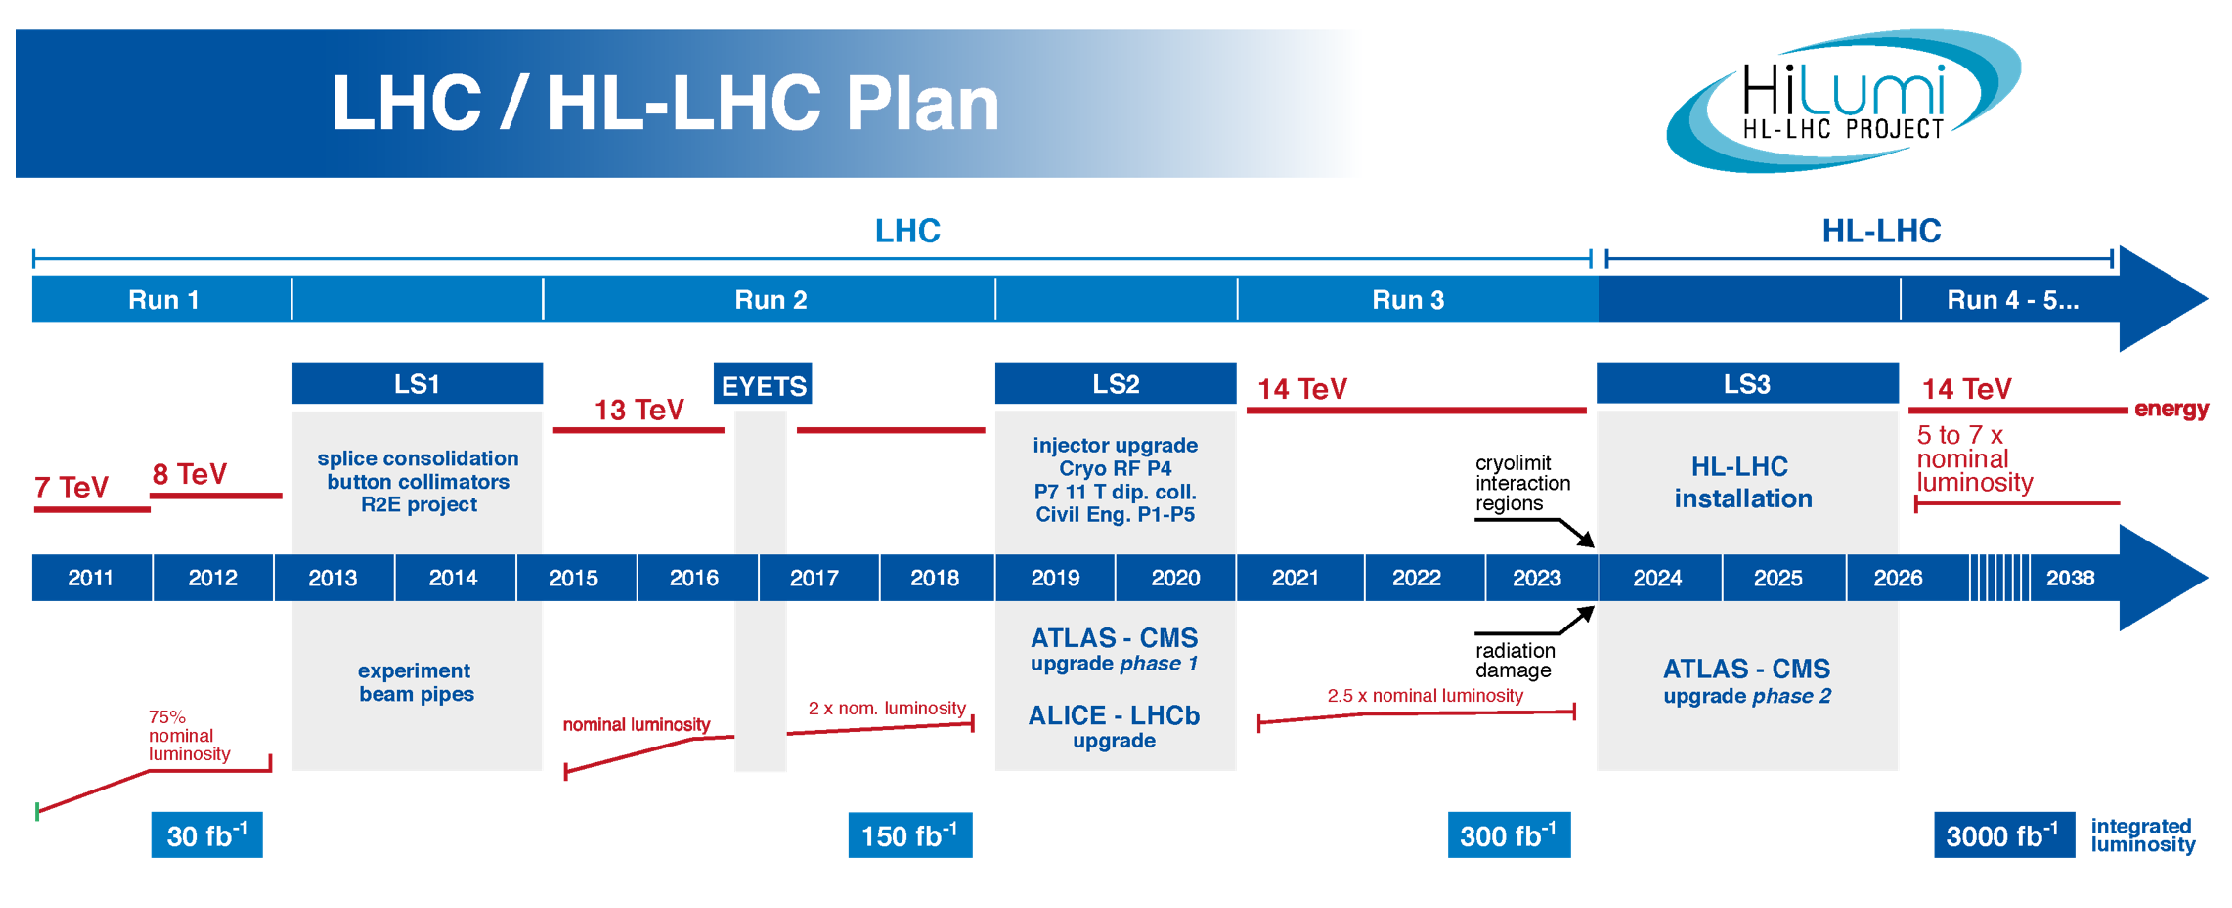
\includegraphics[width=0.9\textwidth]{plots/chapter3/HLLHC.png}
  \caption{Schedule of LHC and HL-LHC operation.}
  \label{fig:HLLHC}
\end{figure}

In order to improve the event reconstruction and enhance its resilience against pileup, the CMS experiment foresees the use of per-particle time information at the level of 30~\ps precision. Combining the time information for electrons and photons with that of charged hadrons widens the physics reach for precise measurements in the Higgs sector and searches of new physics beyond the standard model from simulation studies~\cite{Butler:2019rpu}. As a part of the CMS Phase-2 upgrade, several projects have been proposed, including a new CMS silicon tracker, a new endcap calorimeter, and a minimum ionizing particle timing detector.

The ECAL subdetector needs to be upgraded to maintain its current performance up to the luminosity goals of the LHC Phase-2. As a part of these upgrades, the front-end and off-detector electronics of the EB need to be upgraded along with the complete replacement of the EE~\cite{CMSCollaboration:2015zni}. The primary technical motivation for the upgrade of EB is the Phase-2 trigger requirements to have a latency of 12.5~\mus, compared to the current 4~\mus, and a Level-1 trigger rate of about 750~\khz, compared to the current 100~\khz. In order to meet these requirements, the EB front-end cards and off-detector electronics need to be replaced.

The effect of radiation on lead tungstate crystals has been measured, and it is observed that the scintillation process remains unchanged. However, the formation of scattering color centers affects crystal transparency. The main concern for operating the calorimeter at the HL-LHC is the permanent loss of light transmission due to hadron irradiation. The studies to parametrize and predict the evolution of the crystals under the aging conditions expected at the HL-LHC have been performed at test beam campaigns over the past years~\cite{Adams:2016vi}. By the end of the LHC Phase-2, the energy resolution's constant term is expected to increase to approximately 1.5\% at large $\eta$ in the EB. Thus, the CMS Phase-2 upgrade will retain the EB crystals and the APDs because the constraints measured are compatible with the physics requirements.

The APDs dark current will increase significantly due to the bulk damage of the silicon caused by hadron irradiation. In order to circumvent this and reduce the APD dark current by a factor of 2, the EB operating temperature will be lowered from the nominal Phase-1 $18^\circ \text{C}$ to $9^\circ \text{C}$. With this lowered temperature, it is expected that by the end of the LHC Phase-2, the dark current will reach about 50~\mua (250~\MeV energy-equivalent noise) for APDs at $\aeta = 0$ and about 100~\mua at $\aeta = 1.45$. Figure~\ref{fig:APD} shows the evolution of the dark current for the two operating temperatures, along with a combined scenario where a further lowering of the temperature to $6^\circ \text{C}$ is actuated after about 1600~\fb. The cooling system currently in place will provide sufficient power to stabilize the temperature at $9^\circ \text{C}$. Only minor interventions to the distribution pipes are required to provide chilled water from the surface to the underground cavern and are currently being undertaken during the long LHC shutdown. A more complex modification to the coolant supply system is required for a further temperature reduction step and is still under evaluation.

\begin{figure}[htbp]
  \centering
  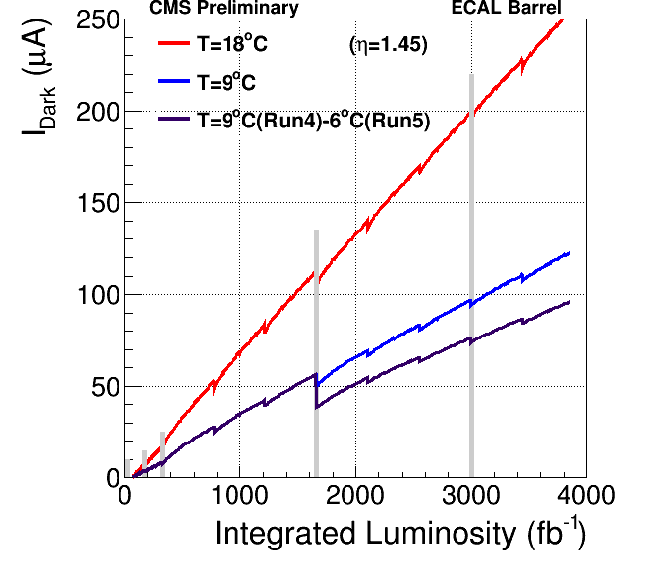
\includegraphics[width=0.6\textwidth]{plots/chapter3/APD.png}
  \caption{APD dark current shown for APDs at $\aeta = 1.45$ operated at $18^\circ \text{C}$ (red curve), at $9^\circ \text{C}$ (blue curve), and in a mixed scenario including a further step to $6^\circ \text{C}$ after the LHC Long Shutdown 4.}
  \label{fig:APD}
\end{figure}

The CMS Phase-2 upgrade will upgrade the very front-end and front-end cards. The upgrade will maintain the mechanical structure of the cooling system and the motherboards. The motherboards are placed below the cooling structure and distribute the low voltage to the electronics and the bias voltage to the photodetectors. They also channel the APD signals to the very front-end cards. A redesigning has been done for the very front-end card to keep low noise and have a shorter pulse shaping and higher sampling rate. A trans-impedance amplifier (TIA) is selected to accomplish this. The TIA generates a voltage image of the photocurrent in the output of the APD, and only the total bandwidth of the system limits the shaping time. The dynamic range of signals up to 2~\TeV is maintained using two gains different by a factor of 10. A lossless data compression algorithm is used to reduce the needed bandwidth for transmitting the TIA signals digitized at 160~\mhz by 12-bit ADCs to the front-end cards.

The front-end card will use new technologies like Low Power Gigabit Transceiver and Versatile Link plus to send single crystal data sampled at 160~\mhz (compared to the current 40~\mhz) to the back-end electronics system. This removes the current requirement of having on-detector data selection and buffering. The data transmitted to the back-end electronics will be processed by the trigger primitive generation algorithm with a crystal level granularity (compared to the current trigger tower level granularity) for usage at the Level-1 trigger. This will increase by a factor of 25 the Level-1 trigger granularity. This also has added benefits in the topological rejection of signals due to direct ionization in the APDs (spikes). Powerful commercially available FPGAs and high-speed optical links will be used in the off-detector electronics. As the electronics are being upgraded, extensive algorithm development is ongoing to test novel algorithms for signal processing, trigger, and data acquisition.

\textbf{Firmware Development:} I took part in the CMS Phase-2 upgrade algorithm development and implemented the trigger primitive generation algorithm for ECAL's proposed Level-1 trigger. ECAL's Level-1 trigger proposal is to perform the trigger primitive generation algorithm in the off-detector electronics and use the crystal-level instead of the tower-level information to calculate the trigger primitives. There are three main stages in which the raw data is processed: linearizer, amplitude filter, and peak finder. During Phase-1 trigger primitive generation, the amplified and digitized signal from 5 crystals of a strip is first linearized. The linearization takes into account the gain and corrects the digitized signal by the calibration coefficients. The amplitude of the strip pulse is measured using the amplitude filter. The filter is based on linear weighted sums, and the weights take into account the expected shape of the signal and subtract the residual pedestal dynamically. This output is then filtered by a peak finder that keeps only the maximum as a measure of the transverse energy contained in the strip.

For Phase-2 trigger primitive generation, the three steps involved are kept the same, except for implementing the algorithm on crystal level digitized signal instead of implementing it on the digitized signal from 5 crystals of a strip. The input to the linearization step is the digitized signal along with the linearizer coefficient. The linearizer coefficient is 24 bits in length. The first 12 bits are the pedestal, subtracted from the digitized signal to get the corrected signal. The next 8 bits are the multiplicative factor applied to the corrected signal to calibrate it. The remaining 4 bits is the bit shift applied to the calibrated signal to get the linearized signal. The amplitude of the linearized signal is estimated using the amplitude filter, which is implemented using a shift register. A shift register is a type of digital circuit using a cascade of flip flops where the output of one flip-flop is connected to the next's input. A 4 stage shift register is used for implementing the amplitude filter, which takes as input the linearized signal along with five weights. The amplitude filter's output is given as input to the peak finder, which is implemented using a 2 stage shift register that finds the peak by comparing the current amplitude output to the previous and next output.

The main challenge for implementing the algorithm lies in the latency constraints. High-Level Synthesis is a tool that converts programs written in high-level programming languages such as C++ into hardware description languages such as VHDL. The algorithm has been implemented using High-Level Synthesis, and the synthesized code is tested on custom hardware (Virtex-7 field-programmable gate array (FPGA)). A clock cycle of $\sim 8.33~\ns$ or 120~\mhz is used for testing the initial implementation of the algorithm. The initiation interval corresponds to the time interval after which the algorithm can read the next input. As the collisions are happening every 25~\ns, the initiation interval is required to be 25~\ns as well. From the synthesis report in Figure~\ref{fig:HLS}, the initiation interval obtained after the algorithm has been synthesized is three clock cycles ($\sim 25~\ns$). Latency corresponds to the time interval from processing the digitized signal to obtaining the peak finder's output. The latency obtained after the algorithm has been synthesized is six clock cycles ($\sim 50~\ns$). The overall resource utilization in the hardware is minimal. In Figure~\ref{fig:HLS}, BRAM corresponds to block random access memory, which is not used, DSP corresponds to digital signal processing, which is used for the multiplication steps by the algorithm, FF corresponds to flip-flops, and LUT corresponds to look-up tables which are used for storage. The DSP usage is 9\%, FF usage is 14\%, while LUT usage is 19\%. This suggests that other algorithms, like multi-fit, spike rejection, etc., can easily be implemented on the hardware as many resources are remaining.

The synthesized VHDL code is converted into a bit file. The bit file contains all of the information necessary to properly configure the device created by our design's implementation tools. The bit file is loaded onto the Virtex-7 FPGA and has been successfully tested. The hardware's output matches the simulation output, which suggests that the algorithm is working as expected. The algorithm implementation has shown the feasibility of using High-Level Synthesis to do the CMS Phase-2 upgrade's firmware development. High-Level Synthesis allows physicists like me to get involved in firmware development using object-oriented languages like C++ without knowing the nitty-gritty details of using hardware description languages like VHDL, which remains in the realm of engineers.

\begin{figure}[htbp]
  \centering
  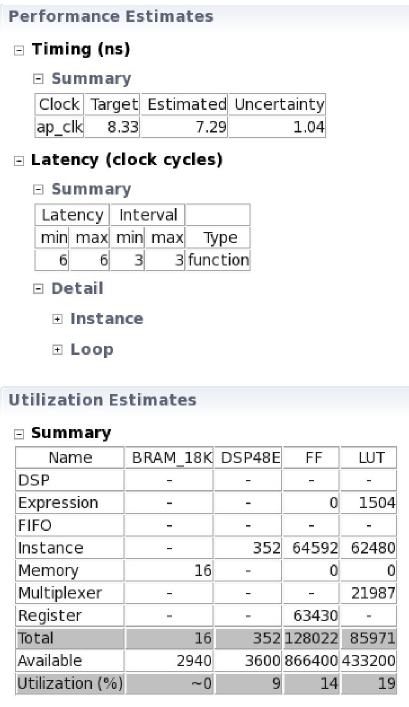
\includegraphics[width=0.6\textwidth]{plots/chapter3/HLS.png}
  \caption{Performance estimates from High-Level Synthesis.}
  \label{fig:HLS}
\end{figure}
